\documentclass[aspectratio=169]{beamer}

\mode<presentation>
{
  \usetheme{default}
  \usecolortheme{default}
  \usefonttheme{default}
  \setbeamertemplate{navigation symbols}{}
  \setbeamertemplate{caption}[numbered]
  \setbeamertemplate{footline}[page number]
  \setbeamercolor{frametitle}{fg=white}
  \setbeamercolor{footline}{fg=black}
} 

\usepackage[english]{babel}
\usepackage[utf8x]{inputenc}
\usepackage{tikz}
\usepackage{listings}
\usepackage{courier}
\usepackage{array}
\usepackage{bold-extra}
\usepackage{minted}
\usepackage[thicklines]{cancel}

\xdefinecolor{darkblue}{rgb}{0.1,0.1,0.7}
\xdefinecolor{darkgreen}{rgb}{0,0.5,0}
\xdefinecolor{darkgrey}{rgb}{0.35,0.35,0.35}
\xdefinecolor{darkorange}{rgb}{0.8,0.5,0}
\xdefinecolor{darkred}{rgb}{0.7,0,0}
\xdefinecolor{dianablue}{rgb}{0.18,0.24,0.31}
\definecolor{commentgreen}{rgb}{0,0.6,0}
\definecolor{stringmauve}{rgb}{0.58,0,0.82}

\lstset{ %
  backgroundcolor=\color{white},      % choose the background color
  basicstyle=\ttfamily\small,         % size of fonts used for the code
  breaklines=true,                    % automatic line breaking only at whitespace
  captionpos=b,                       % sets the caption-position to bottom
  commentstyle=\color{darkorange},  % comment style
  escapeinside={\%*}{*)},             % if you want to add LaTeX within your code
  keywordstyle=\color{blue},          % keyword style
  keywordstyle=[2]\color{stringmauve},          % keyword style
  keywordstyle=[3]\color{darkgreen},          % keyword style
  stringstyle=\color{stringmauve},    % string literal style
  showstringspaces=false,
  showlines=true
}

\lstdefinelanguage{femtocode}{
  keywords = [2]{histogram,filter,distinctpairs,table,map,flatten},%
  keywords = [3]{tracks,calorimeterEnergy,trackMomentum,outerHits,charge},%
  morekeywords={def,and},
  otherkeywords={=>,<-,<\%,<,>,/,*,:,\#,@},
  sensitive=true,
  comment=[l]{\#},
  morestring=[b]",
  morestring=[b]',
  morestring=[b]"""
}

\title[2017-09-29-strangeloop]{Particle Physics, 10\,000 times faster}
\author{Jim Pivarski}
\institute{Princeton University -- DIANA}
\date{September 30, 2017}

\begin{document}

\logo{\pgfputat{\pgfxy(0.11, 7.4)}{\pgfbox[right,base]{\tikz{\filldraw[fill=dianablue, draw=none] (0 cm, 0 cm) rectangle (50 cm, 1 cm);}
\includegraphics[height=1 cm]{diana-hep-logo.png}}}}

\begin{frame}
  \titlepage
\end{frame}

% Uncomment these lines for an automatically generated outline.
%\begin{frame}{Outline}
%  \tableofcontents
%\end{frame}

%%%%%%%%%%%%%%%%%%%%%%%%%%%%%%%%%%%%%%%%%%%%%%%%%%%%%%%

%%%% START

\begin{frame}{Particle physics: the most industrial field of academia}
\vspace{0.15 cm}
\begin{columns}
\column{0.37\linewidth}
\begin{center}
\begin{minipage}{0.8\linewidth}

\textcolor{darkblue}{The goals are academic:} to explore strange new phenomena; to seek out new particles and new \mbox{interactions\ldots}

\vspace{0.5 cm}
\textcolor{darkblue}{The scale is industrial:} \mbox{billion} dollar hardware, planning on decadal time- scales, \mbox{millions} of lines of code\ldots

\vspace{0.5 cm}
\end{minipage}
\end{center}

\column{0.77\linewidth}
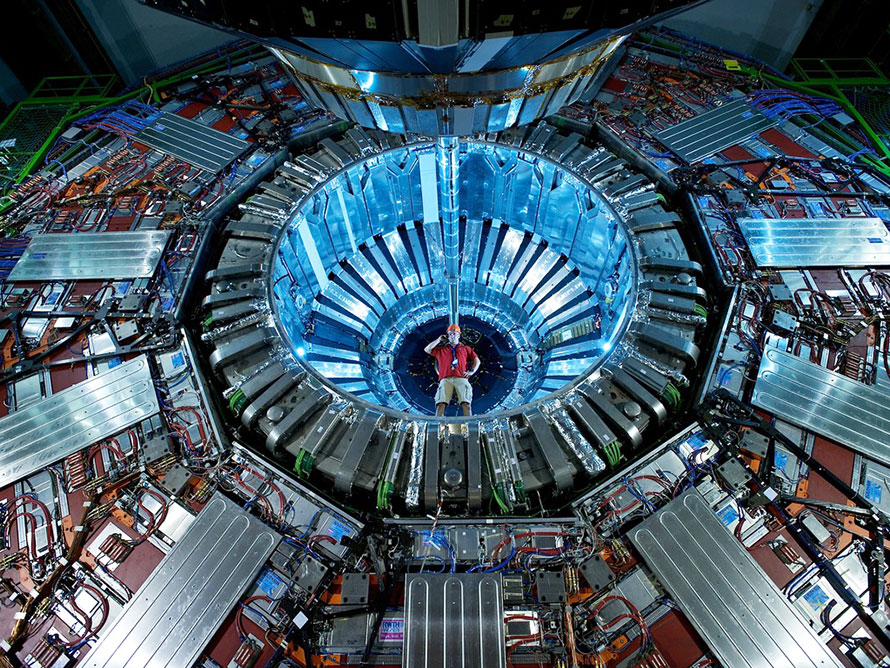
\includegraphics[width=\linewidth]{lhc-industrial-2.jpg}

\end{columns}
\end{frame}

\begin{frame}{It's big data\ldots\ \only<2->{but not {\it really} big}}
\vspace{0.35 cm}
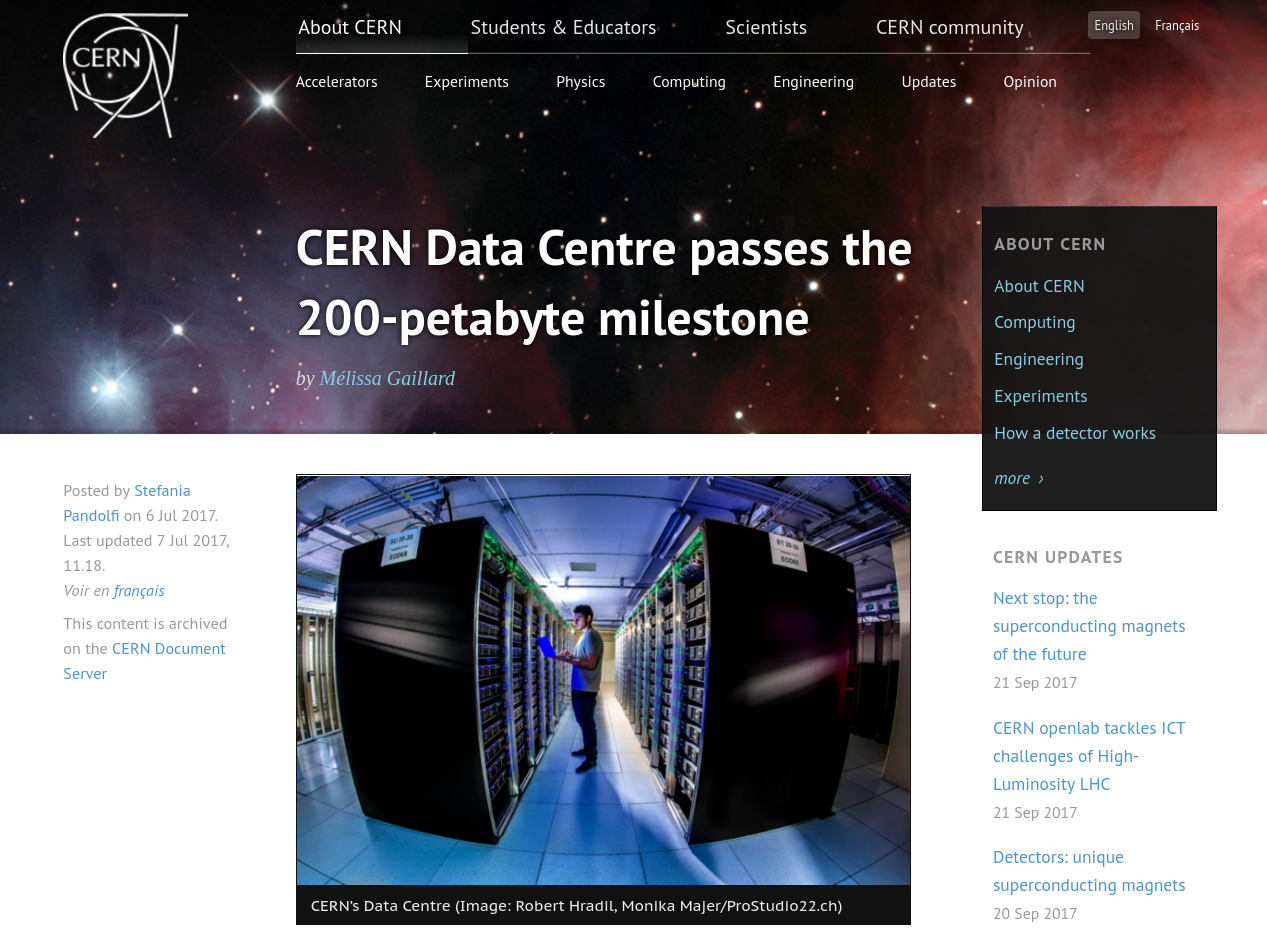
\includegraphics[width=0.73\linewidth]{cern-200pb.png}

\vspace{-4.8 cm}
\uncover<2->{\mbox{ } \hfill 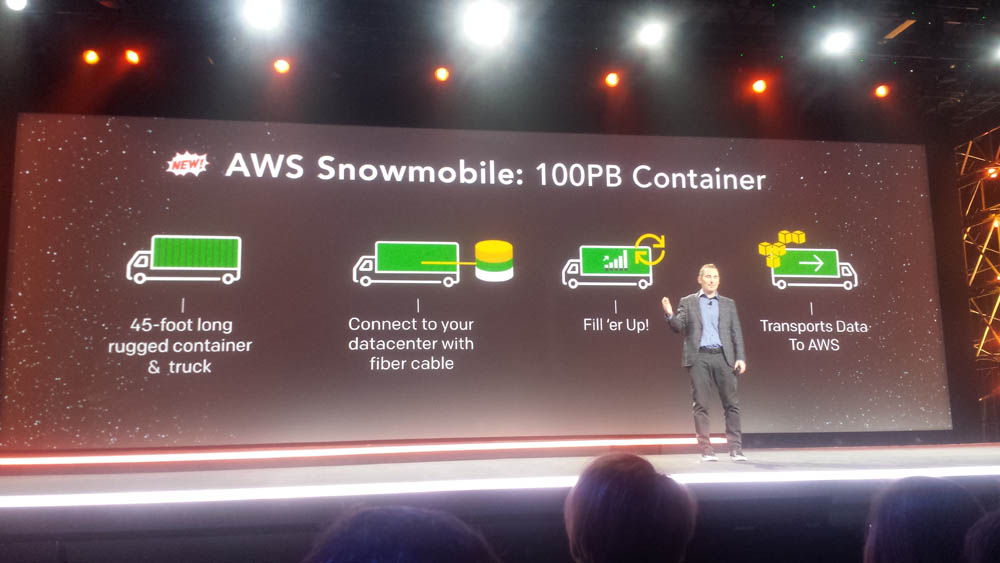
\includegraphics[width=0.7\linewidth]{aws-snowmobile.jpg}\hspace{-1 cm}}
\end{frame}

\begin{frame}{It will be getting bigger\ldots}
\begin{center}
\only<1>{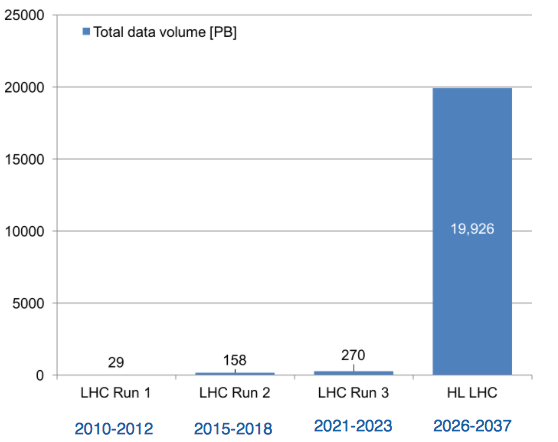
\includegraphics[width=0.7\linewidth]{the-coming-flood.png}}
\only<2>{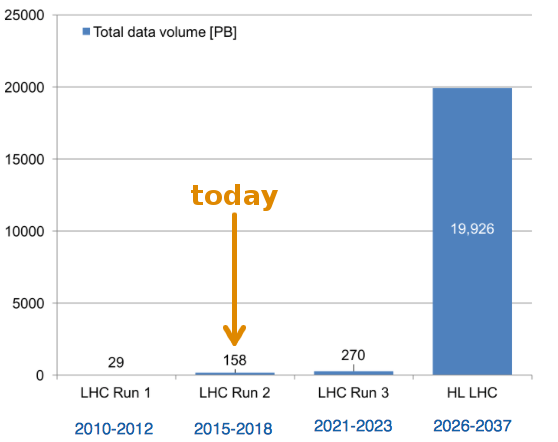
\includegraphics[width=0.7\linewidth]{the-coming-flood-2.png}}
\end{center}
\end{frame}

\begin{frame}{Our software developed \only<1>{outside}\only<2->{\xcancel{outside} \underline{before}} the big data ecosystem}
\vspace{0.5 cm}
\begin{uncoverenv}<3->
\fbox{\begin{minipage}{5 cm}
It's my job to try to find ways to bridge the divide.
\end{minipage}}
\end{uncoverenv}

\vspace{-1.43 cm}
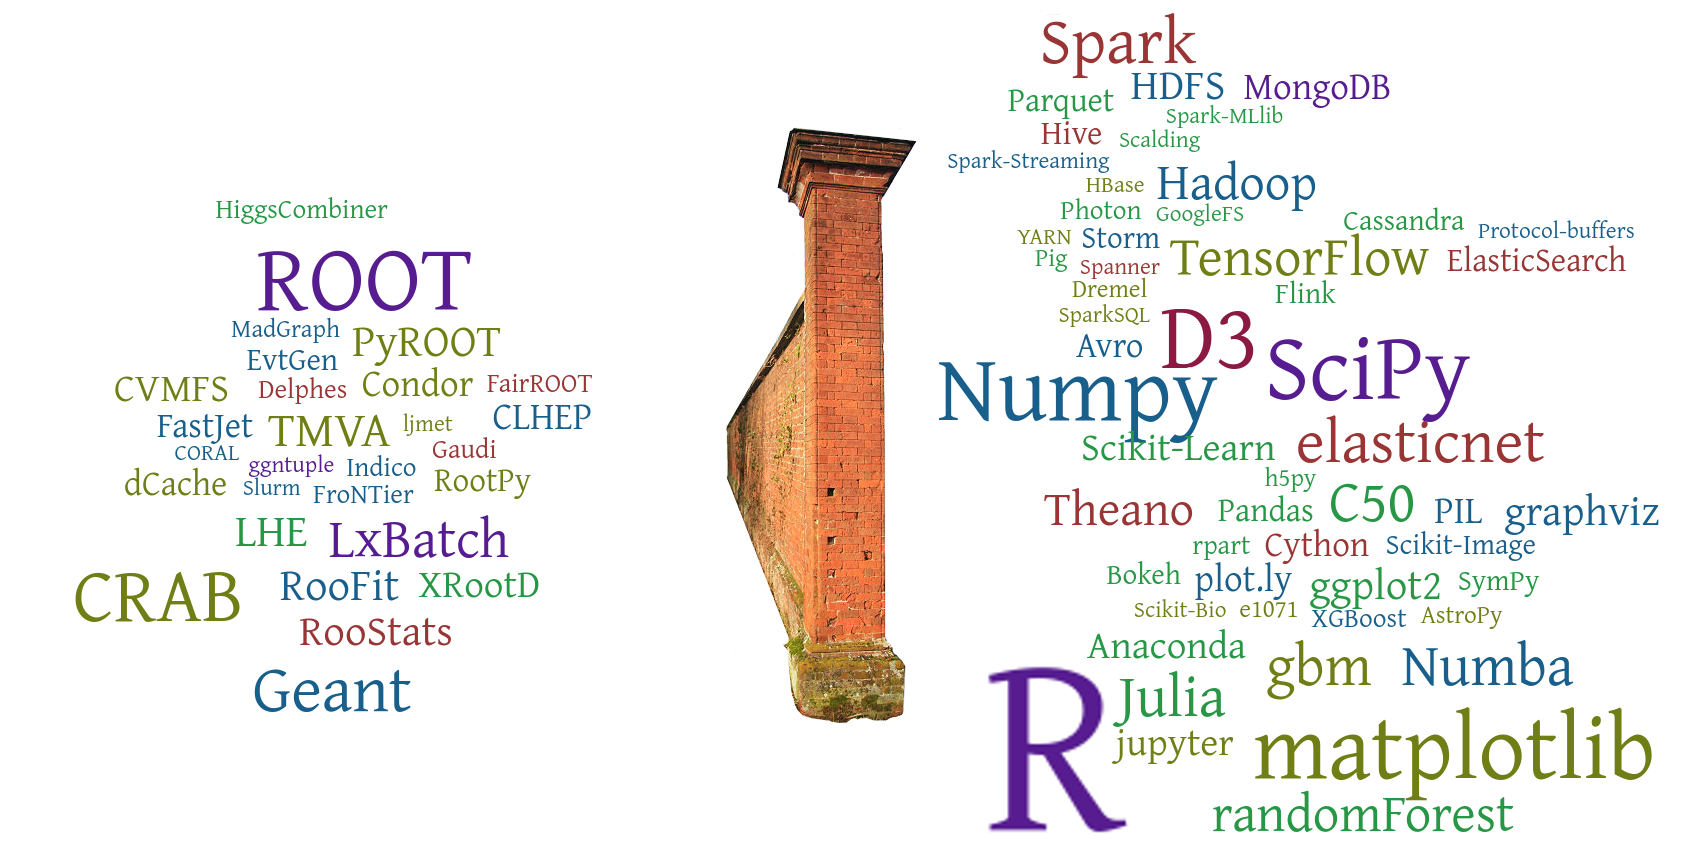
\includegraphics[width=\linewidth]{separation.png}
\end{frame}

\begin{frame}{}
\vspace{1 cm}
\large
\begin{center}
The obstacles are not just {\it accidental}--- artifacts of technology choice \\ (e.g.\ C++ in particle physics and Java in the Hadoop/Spark world).

\vspace{1 cm}
There are also {\it essential} qualities that current big data systems don't offer.

\vspace{1 cm}
\uncover<2->{\textcolor{darkblue}{This represents an opportunity on both sides: alien civilizations that evolved independenly can learn a lot from each other!}}
\end{center}
\end{frame}

\begin{frame}{So, what is unique about particle physics data?}

\begin{columns}
\column{1.15\linewidth}
\vspace{0.11 cm}
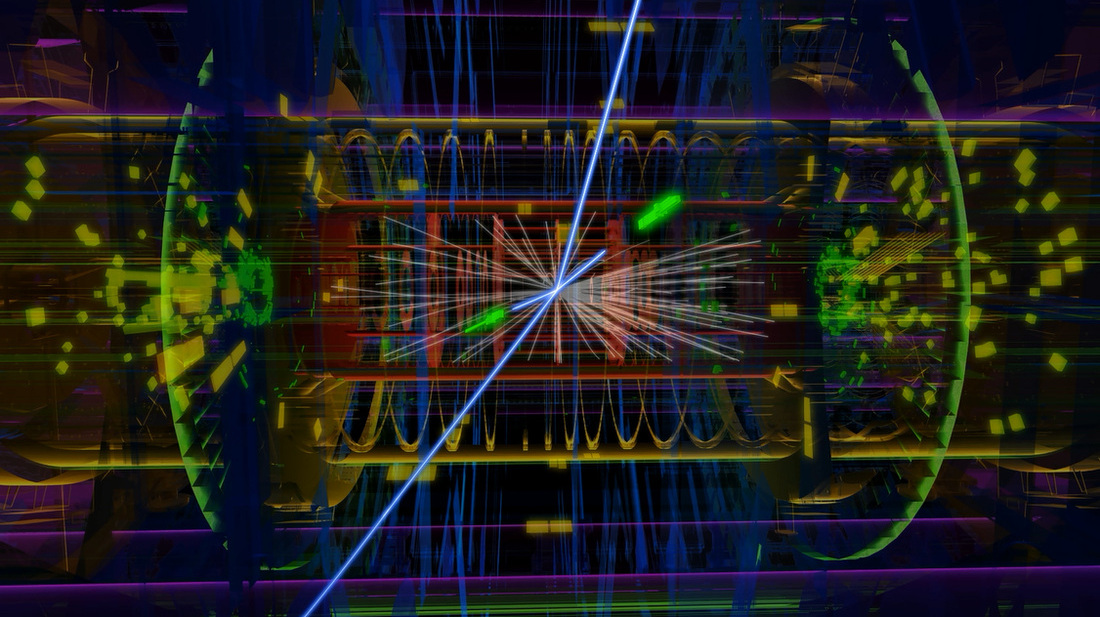
\includegraphics[width=\linewidth]{complex-atlas-collision-art.jpg}
\end{columns}

\vspace{-8.7 cm}
\uncover<2->{\textcolor{white}{\huge\bf It's not the size (100's of PB).}}

\vspace{0.5 cm}
\uncover<3->{\textcolor{white}{\huge\bf Arguably, it's the \underline{complexity}.}}

\vspace{3.9 cm}
\uncover<4->{\textcolor{white}{\huge\bf This picture represents one ``row'' in our data ``table.''}}

\vspace{8.7 cm}
\end{frame}

\begin{frame}{``Row'' and ``table'' in quotation marks\ldots}
\vspace{0.75 cm}
\textcolor{darkblue}{\LARGE Particle physics data are not stored in databases.}

\vspace{0.5 cm}
\begin{itemize}\setlength{\itemsep}{0.5 cm}
\item<2-> We don't benefit from indexing, query planning, or high-level query languages.
\item<3-> Every data pull is a custom C++ program, accessing lists of files, taking months while the user chases down failures and stragglers.
\item<4-> But if our data {\it were} in a conventional (relational or NoSQL) database, the first thing we'd do is extract it and work with files again.
\end{itemize}
\begin{center}
\huge \uncover<5->{Why?}
\end{center}
\end{frame}

\begin{frame}
\vspace{0.5 cm}
\begin{columns}[t]
\column{0.5\linewidth}
\begin{center}
\Large Our data are deeply nested \\ and cross-linked

\vspace{-0.25 cm}
\rule{\linewidth}{0.8 pt}
\end{center}

\vspace{-0.25 cm}
\begin{itemize}\setlength{\itemsep}{0.5 cm}
\item<2-> Not a problem nowadays, as Drill, Parquet, and Arrow can explode nested structures into columns for fast, sparse access.

\vspace{0.2 cm}
\textcolor{gray}{(We've been doing it since the 90's.)}

\item<3-> Cross-links (pointers) could be supported by a graph database.

\vspace{0.2 cm}
\textcolor{gray}{(Though list indexes work well enough for our large number of small graphs.)}

\end{itemize}

\column{0.5\linewidth}
\begin{center}
\Large The operations we perform make intensive use of that structure

\vspace{-0.25 cm}
\rule{\linewidth}{0.8 pt}
\end{center}

\vspace{-0.25 cm}
\begin{itemize}
\item<4-> We frequently need to search sublists under constraints, optimize pairings, iterate over combinatorics\ldots

\item<5-> Even the simplest particle physics search criteria would require explodes, tags, and joins in SQL.

\vspace{0.5 cm}
\begin{uncoverenv}<6->
\fbox{\begin{minipage}{\linewidth}
To give a sense of the problem, I'll walk through the steps of an analysis.
\end{minipage}}
\end{uncoverenv}
\end{itemize}
\end{columns}
\end{frame}

\begin{frame}{From raw signals to tracks}
\vspace{0.15 cm}
\begin{columns}[b]
\column{0.515\linewidth}
\hspace{-0.5 cm}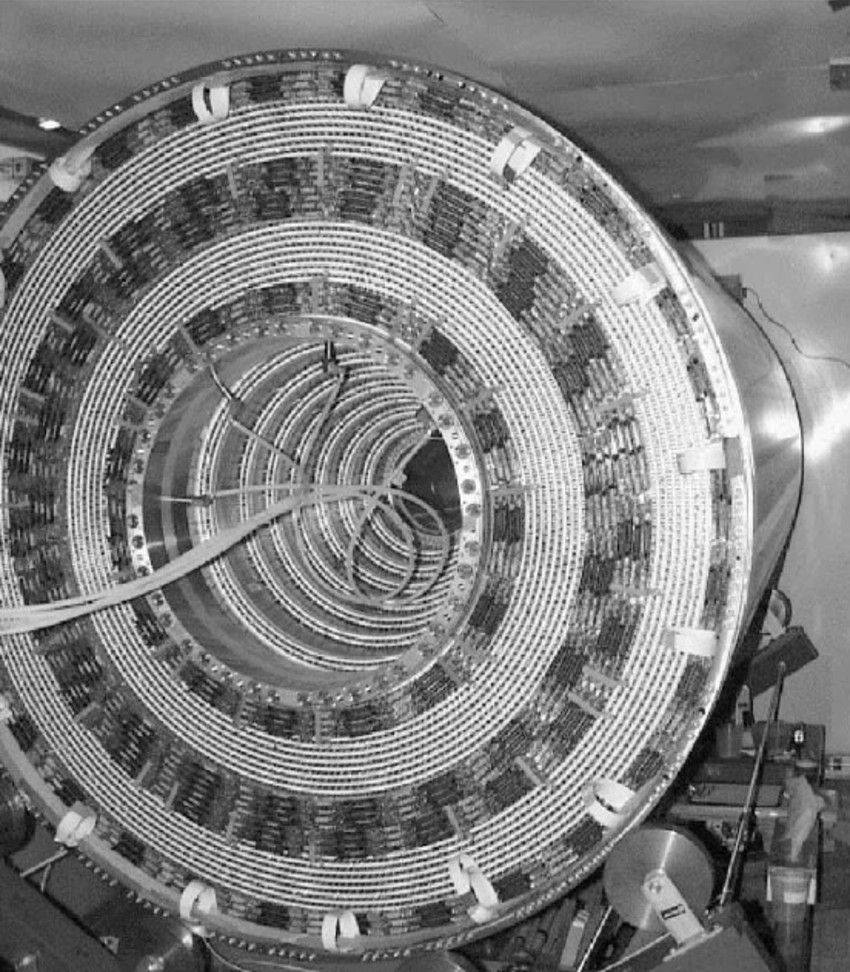
\includegraphics[width=\linewidth]{cleoiii.jpg}

\only<1-4>{\vspace{0.75 cm}}

\column{0.55\linewidth}
\begin{onlyenv}<1,2,6>
\mbox{\hspace{-0.5 cm}\begin{minipage}{0.95\linewidth}
\only<1>{Can you see the particle tracks?}
\only<2>{How about now?}
\only<6>{Raw data could have been a (sparsely filled) table, but tracks are an arbitrary-length list of objects.}

\vspace{-1 cm}
\end{minipage}}
\end{onlyenv}

\vspace{0.25 cm}
\only<1>{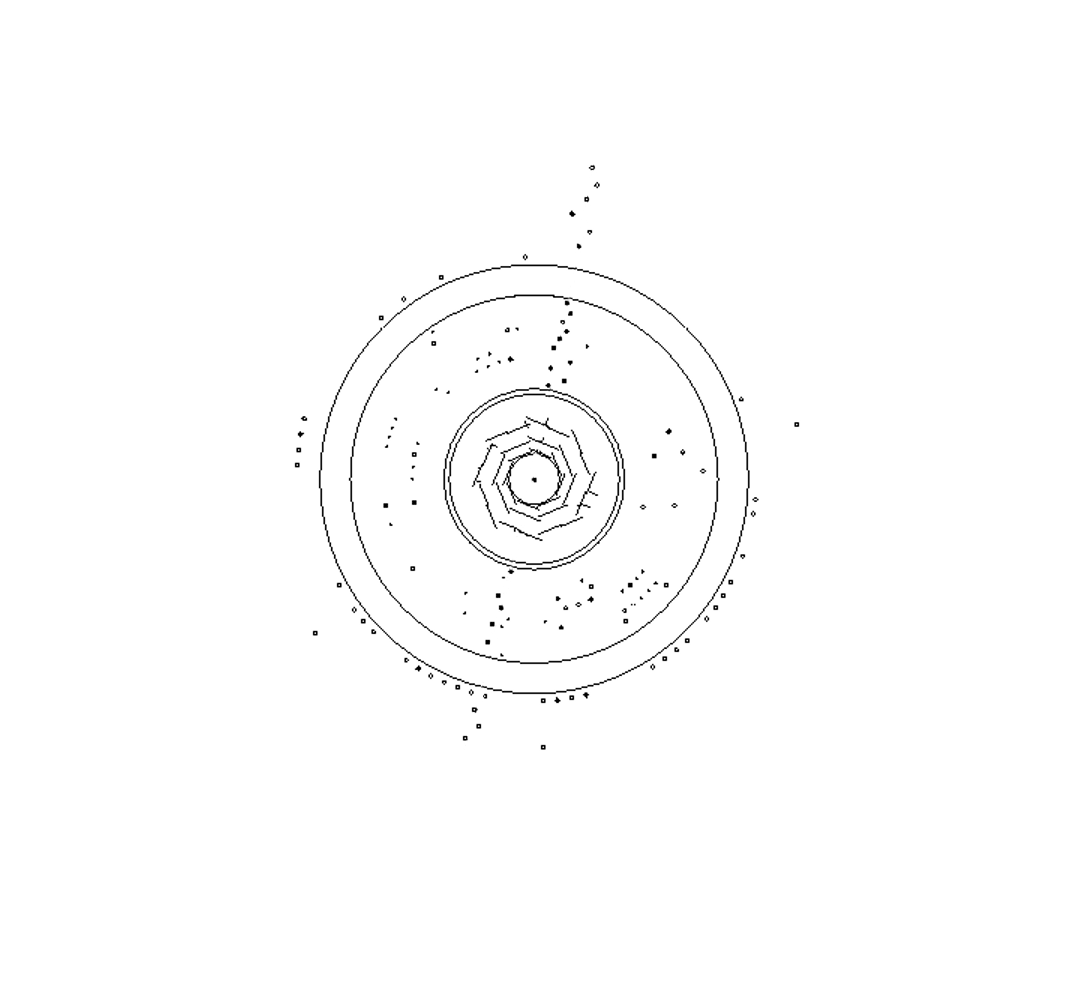
\includegraphics[width=\linewidth]{tracking-1.png}}
\only<2>{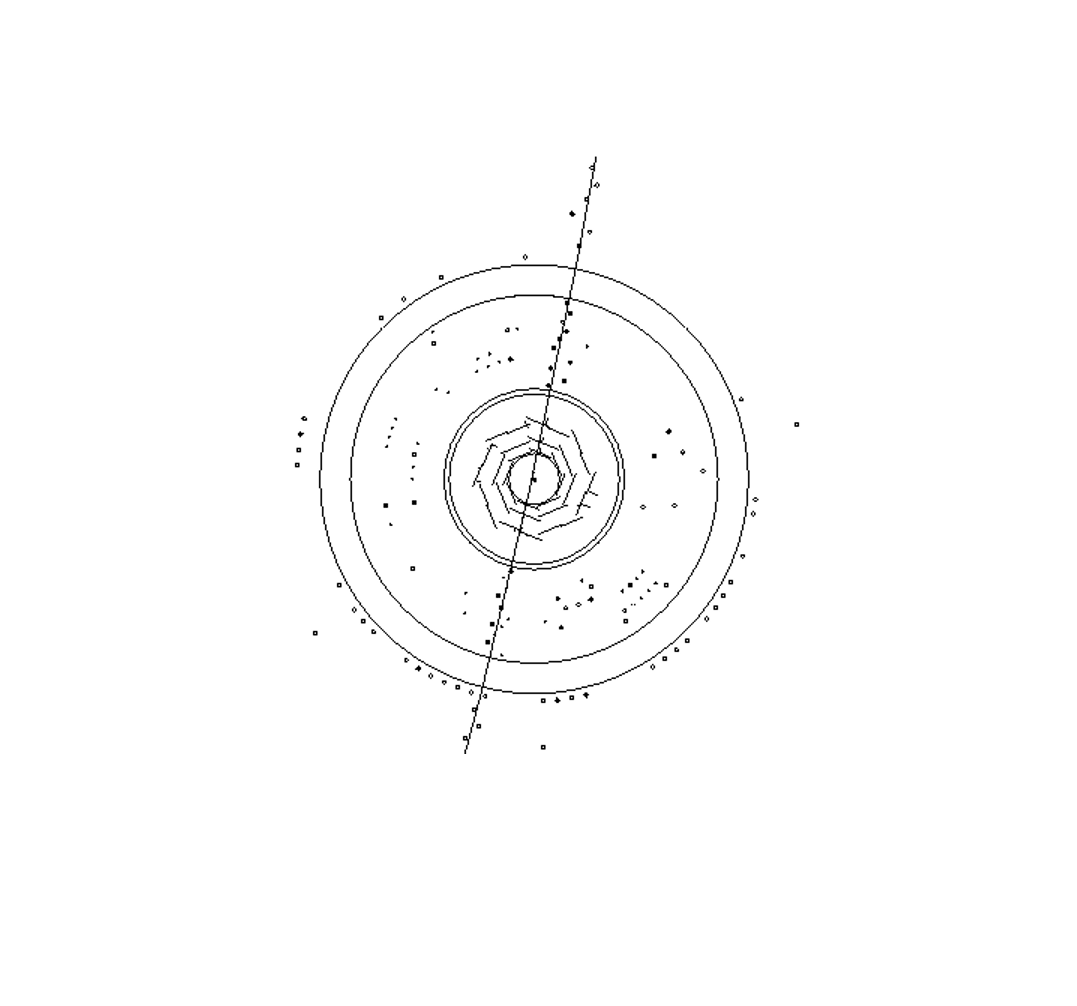
\includegraphics[width=\linewidth]{tracking-2.png}}
\only<3>{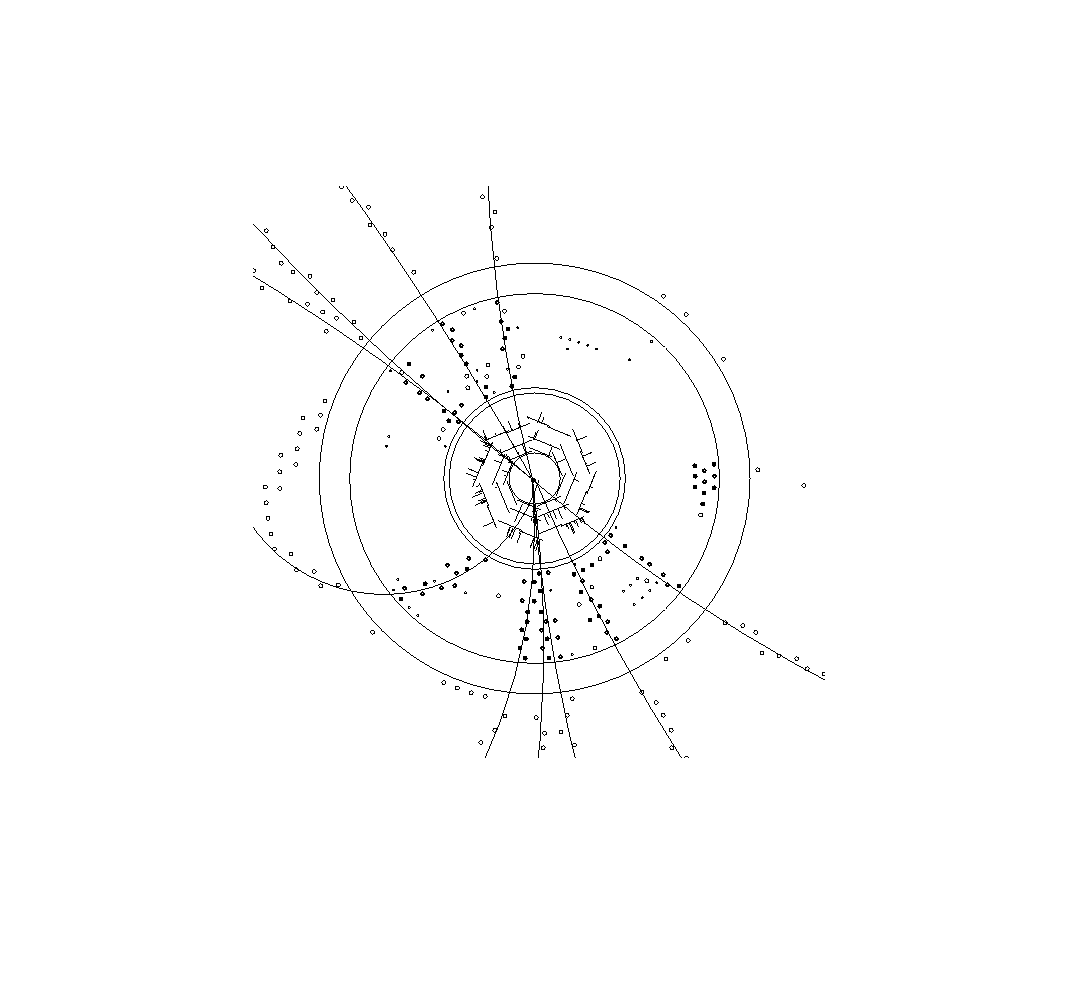
\includegraphics[width=\linewidth]{tracking-3.png}}
\only<4>{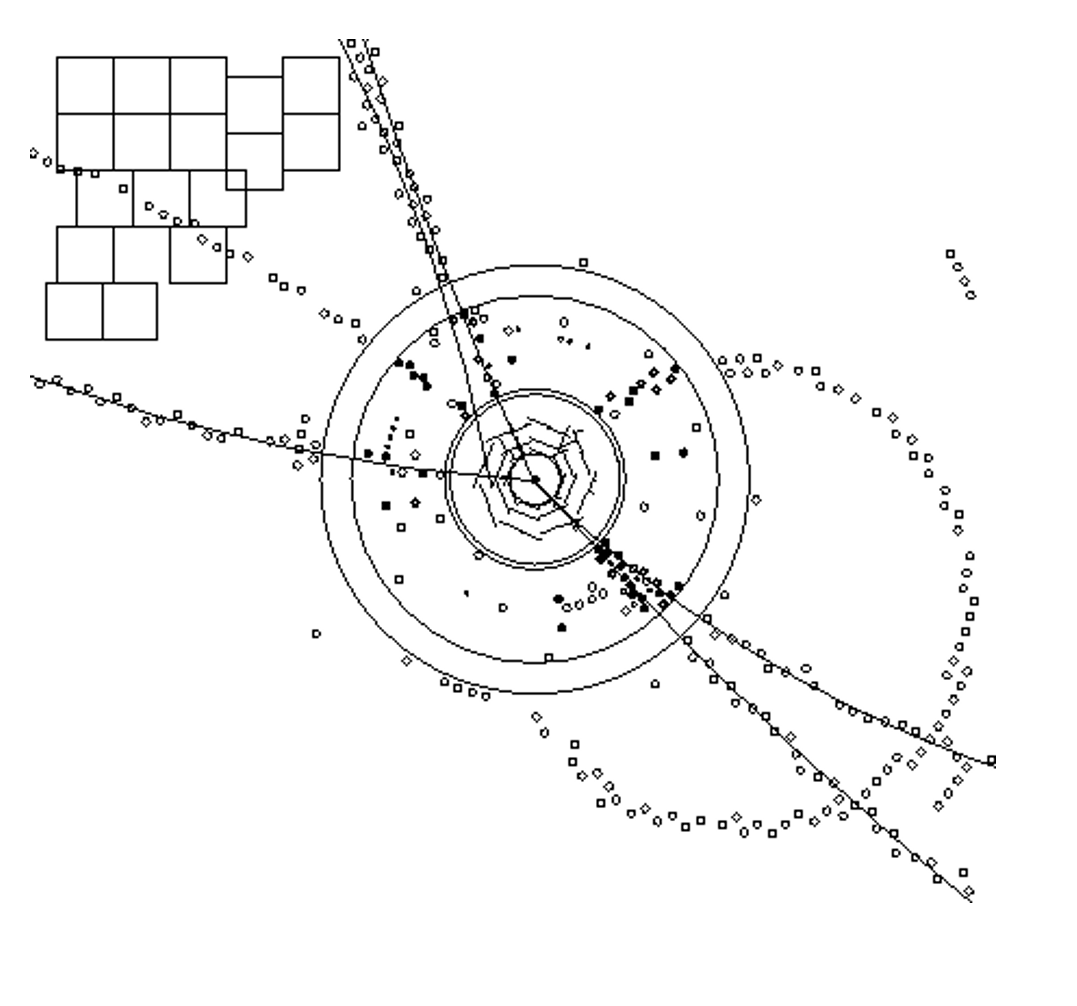
\includegraphics[width=\linewidth]{tracking-4.png}}
\only<5>{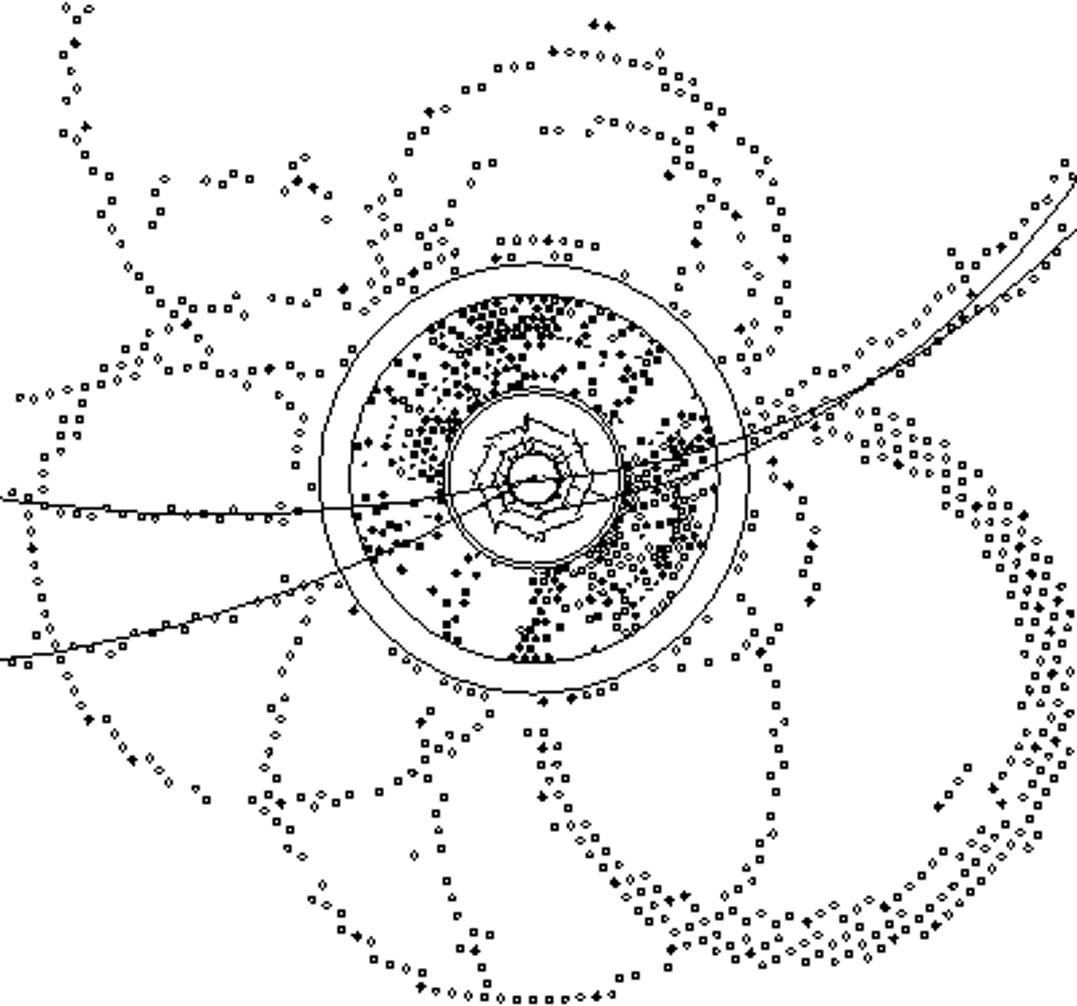
\includegraphics[width=\linewidth]{tracking-5.png}}
\only<6>{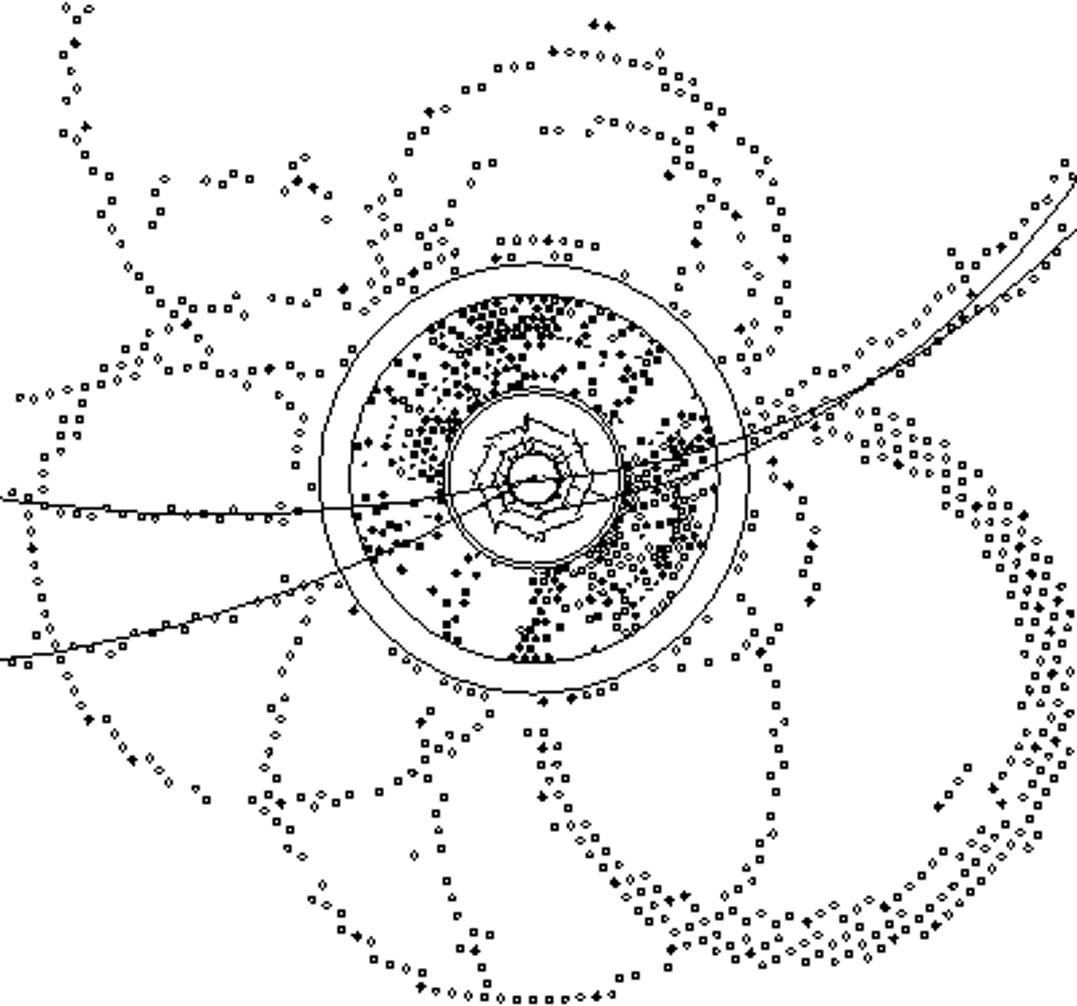
\includegraphics[width=\linewidth]{tracking-6.png}}

\only<1-4>{\vspace{0.25 cm}}
\vspace{0.25 cm}
\end{columns}
\end{frame}

\begin{frame}{From tracks to particles}
\vspace{0.25 cm}
Tracks are long-lived particles (on the nanosecond scale) that came from the decay of very short-lived particles.

\vspace{-0.5 cm}
\begin{center}
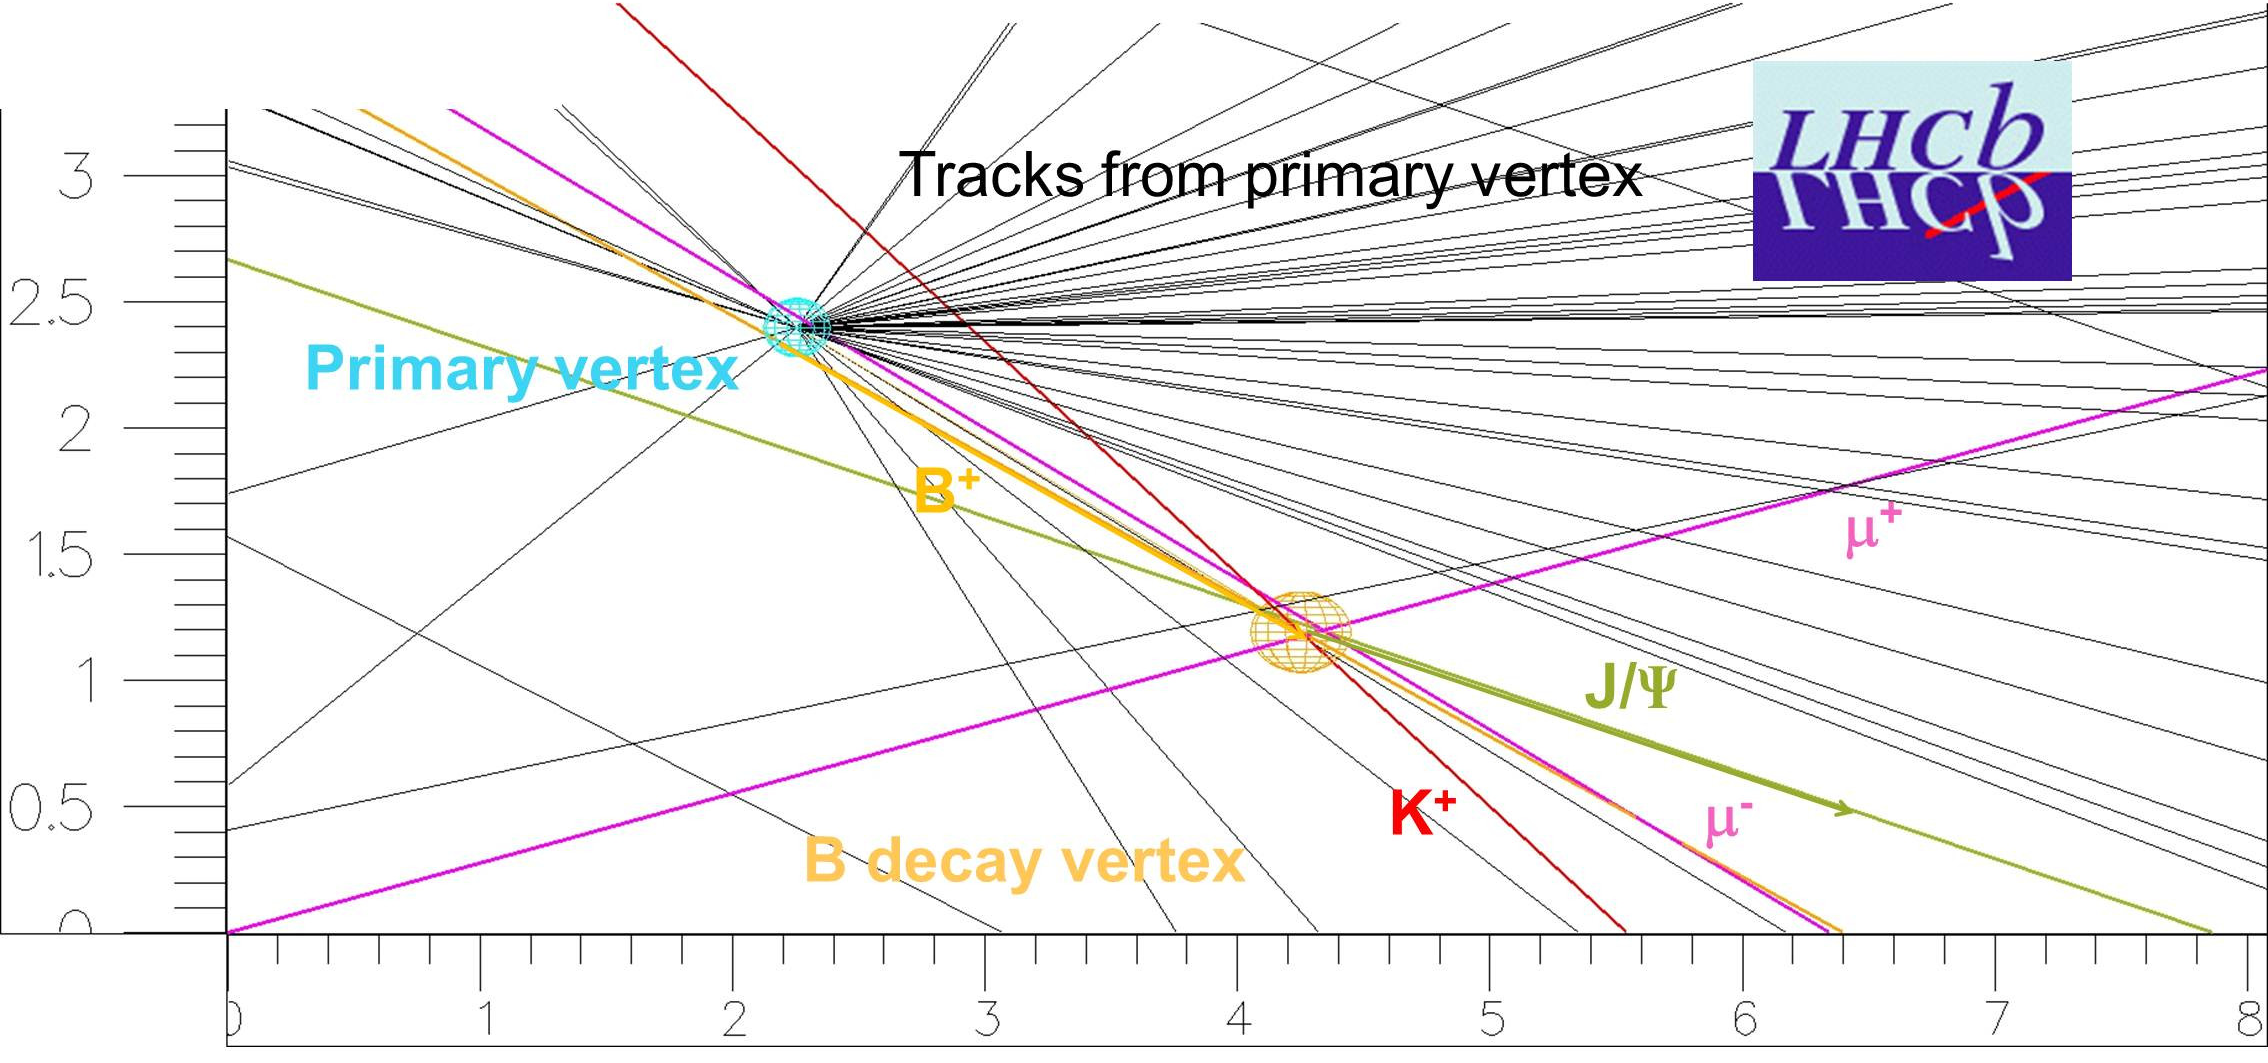
\includegraphics[width=0.9\linewidth]{lhcb.png}
\end{center}

\vspace{-0.25 cm}
Tracks have structured associations with one another, and those associations are not certain: flexibility has to be carried through to the final analysis.
\end{frame}

\begin{frame}{And there are a lot of combinations to consider\ldots}
\vspace{0.15 cm}
\begin{columns}
\column{1.2\linewidth}
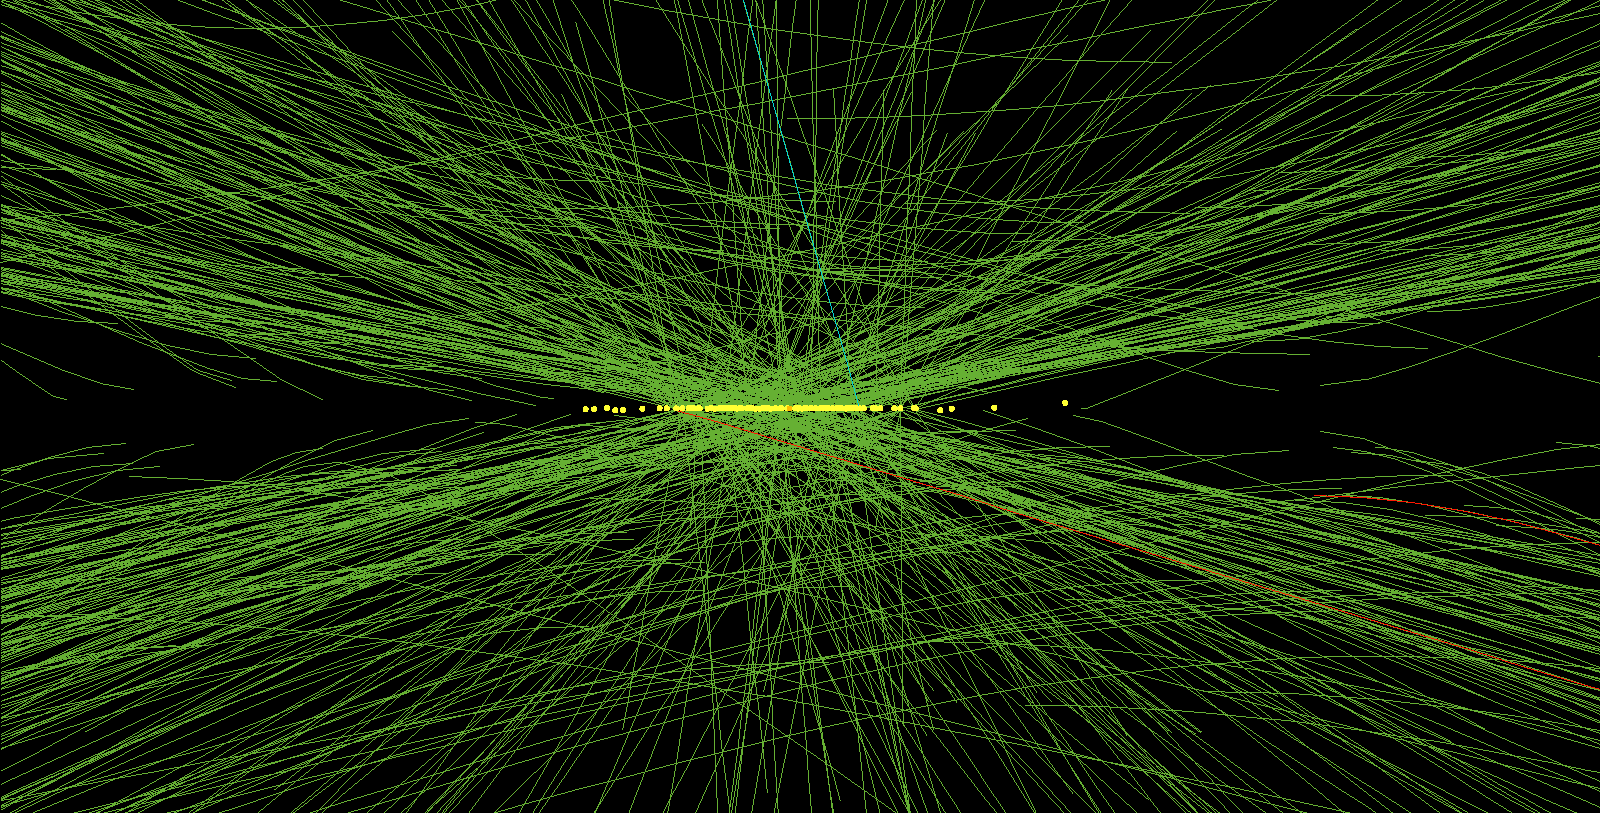
\includegraphics[width=\linewidth]{pileup.png}
\end{columns}
\end{frame}

\begin{frame}{From particles to discovery}
\vspace{0.25 cm}
\mbox{\hspace{0.25 cm}\begin{columns}[b]
\column{0.6\linewidth}
Suppose there's a particle called ``Higgs'' that would decay into two ``Z bosons,'' each of which decays into two electrons or two muons.

\only<1-5>{\[ H \to ZZ \to \vphantom{\mu^+}e^+e^-\mu^+\mu^- \]}
\only<6>{\[ H \to ZZ \to \underbrace{\vphantom{\mu^+}e^+e^-}\mu^+\mu^- \]}
\only<7>{\[ H \to ZZ \to \underbrace{\vphantom{\mu^+}e^+e^-}\underbrace{\mu^+\mu^-} \]}
\only<8->{\[ H \to ZZ \to \underbrace{\hspace{0.33 cm}\underbrace{\vphantom{\mu^+}e^+e^-}\hspace{0.33 cm}\underbrace{\mu^+\mu^-}\hspace{0.33 cm}}_{\mbox{\scriptsize compute mass of progenitor}} \]}

\begin{center}
\only<1-8>{\vspace{2 cm}}
\only<9>{\vspace{-0.25 cm}}
\only<9>{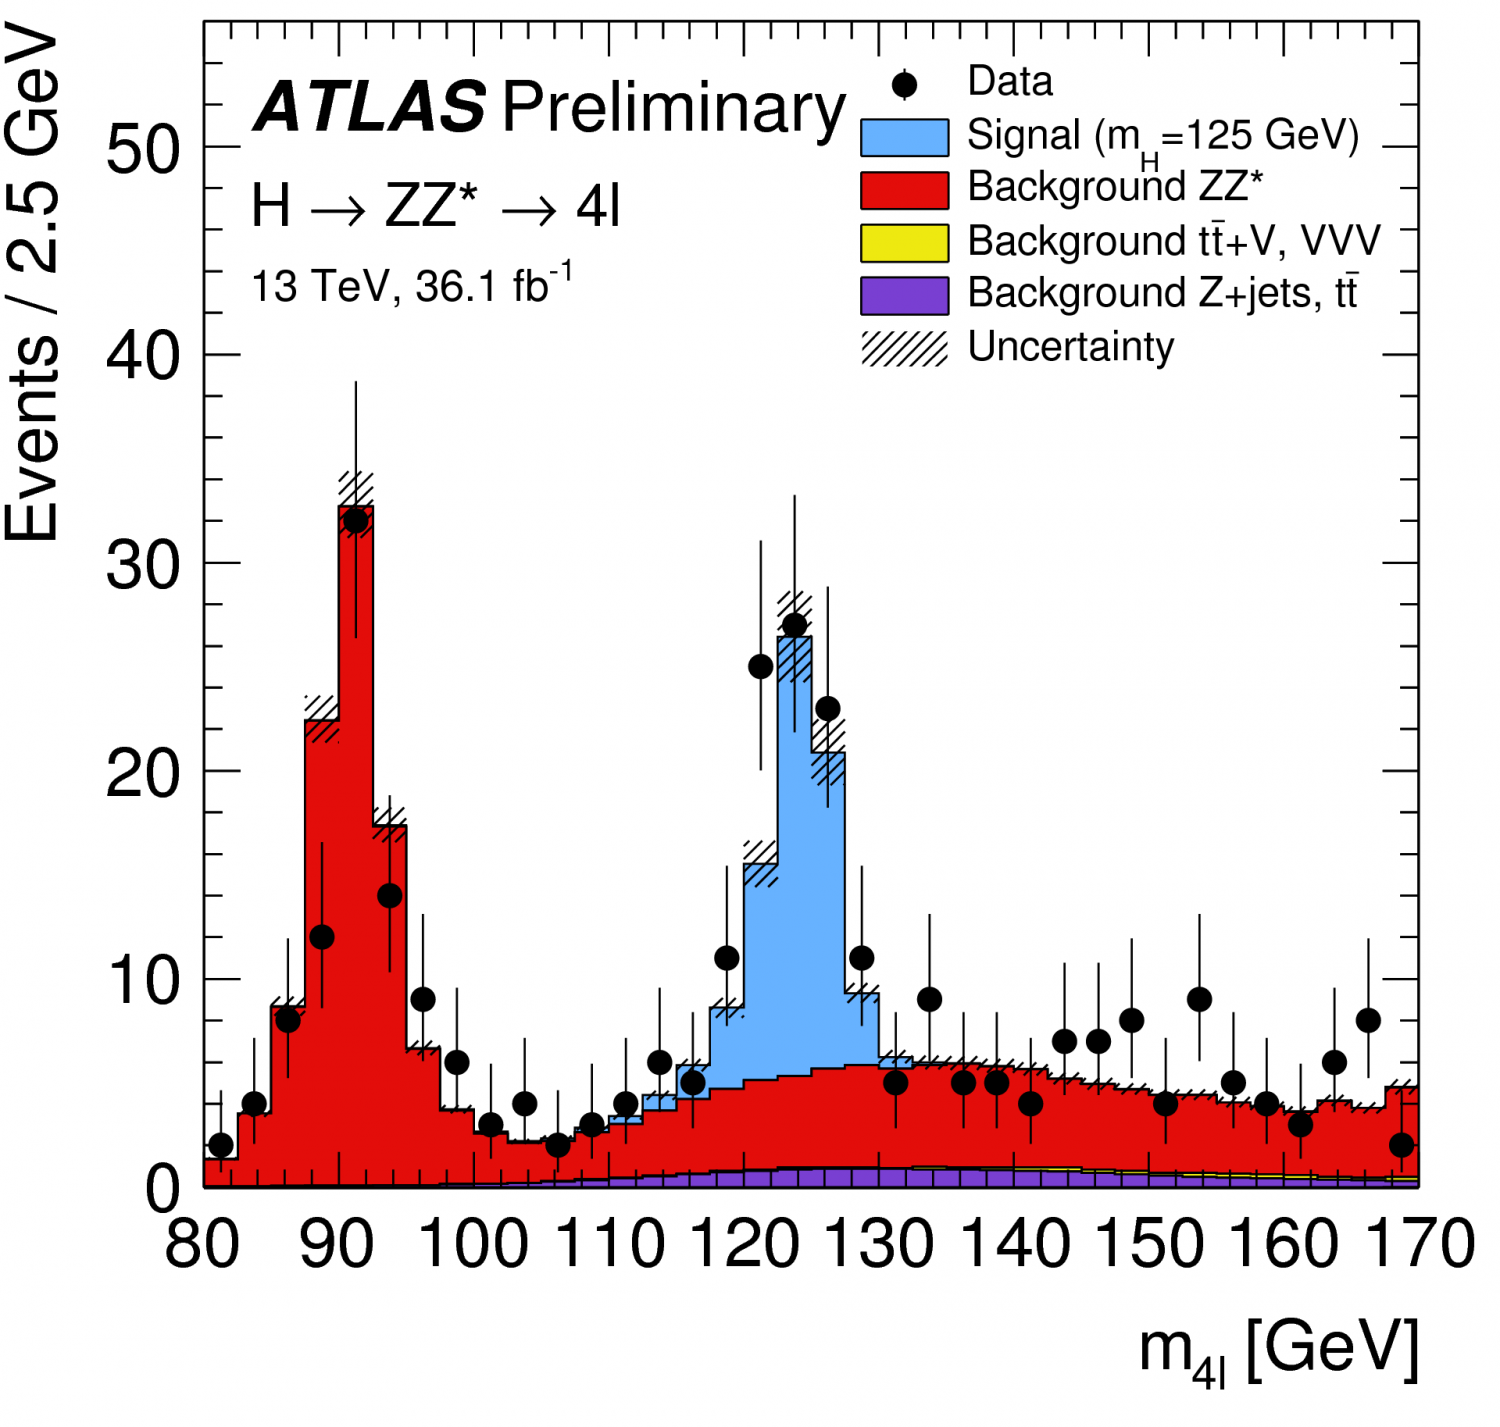
\includegraphics[width=0.55\linewidth]{atlas-higgs.png}}
\end{center}

\only<1-3>{\vspace{0.05 cm}}
\column{0.45\linewidth}
\vspace{0.1 cm}
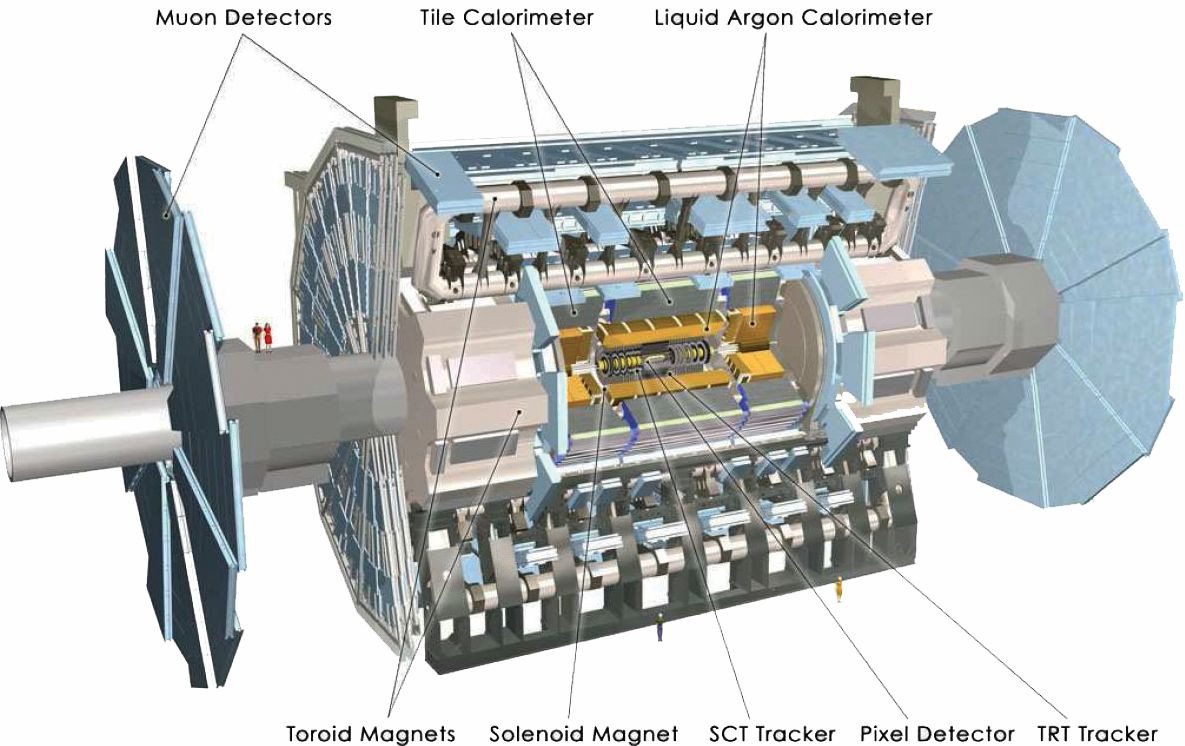
\includegraphics[width=\linewidth]{atlas-detector.jpg}

\vspace{0.15 cm}
\only<1>{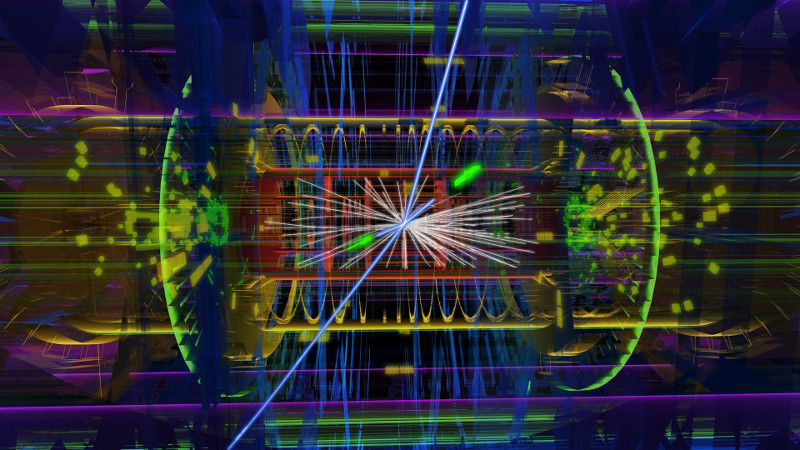
\includegraphics[width=\linewidth]{complex-atlas-collision-science-1.jpg}}
\only<2>{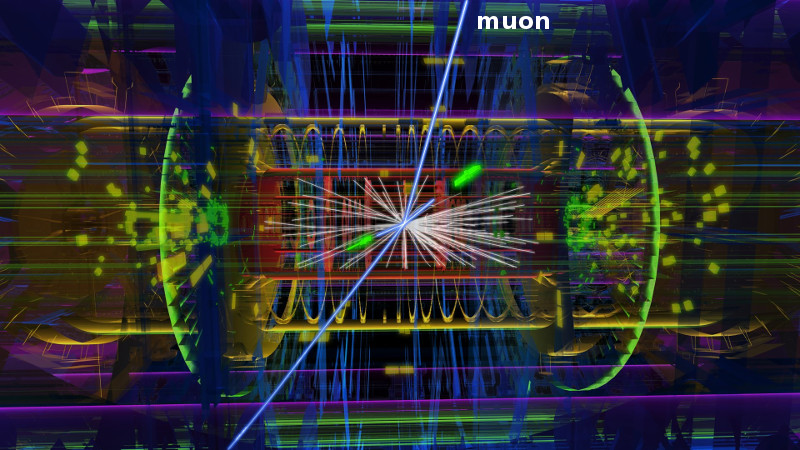
\includegraphics[width=\linewidth]{complex-atlas-collision-science-2.jpg}}
\only<3>{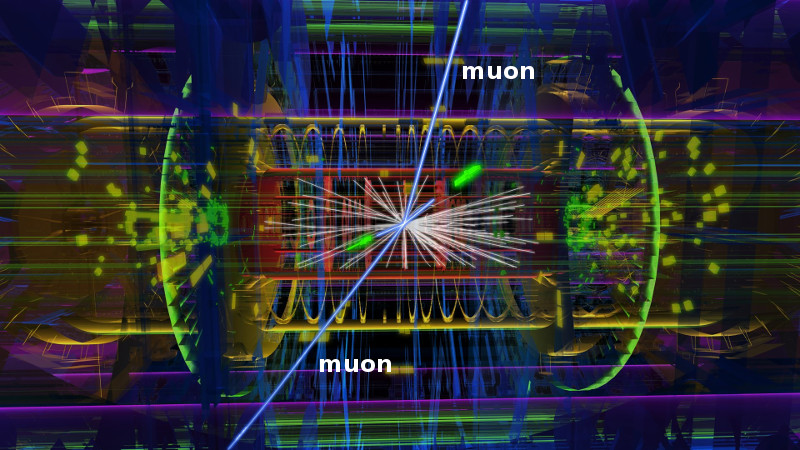
\includegraphics[width=\linewidth]{complex-atlas-collision-science-3.jpg}}
\only<4>{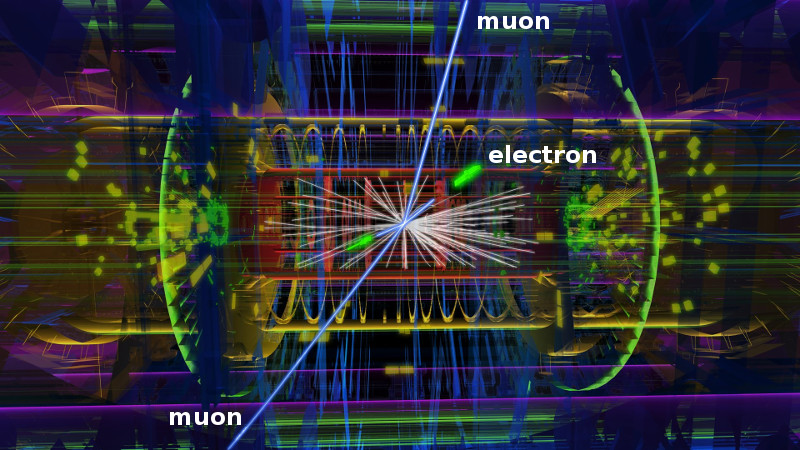
\includegraphics[width=\linewidth]{complex-atlas-collision-science-4.jpg}}
\only<5->{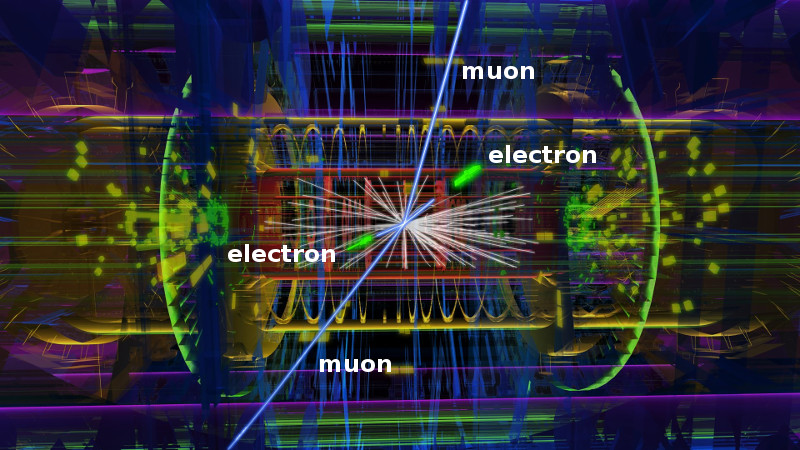
\includegraphics[width=\linewidth]{complex-atlas-collision-science-5.jpg}}
\end{columns}}
\end{frame}

\begin{frame}{Objects versus flat tables}
\vspace{0.5 cm}
\begin{columns}[b]
\column{0.5\linewidth}
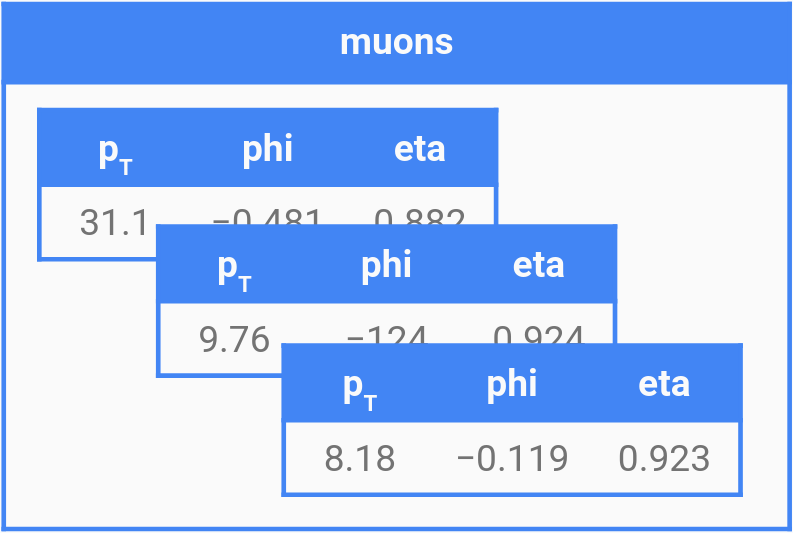
\includegraphics[width=\linewidth]{muons-as-objects.png}

\column{0.5\linewidth}
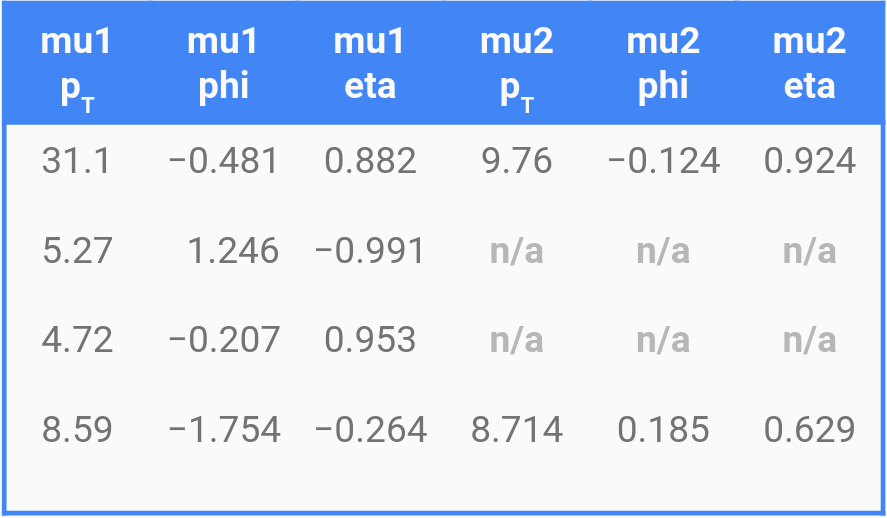
\includegraphics[width=\linewidth]{muons-as-a-table.png}
\vspace{0.61 cm}
\end{columns}

\vspace{0.2 cm}
To try different associations between particles, between data from different detectors, in many different combinations\ldots

\vspace{0.2 cm}
\hfill \textcolor{darkblue}{\ldots it's easier to write these as algorithms over {\it objects.}}
\end{frame}

\begin{frame}[fragile]{Modern SQL can {\it represent} that}
\vspace{0.5 cm}
\begin{columns}
\column{0.4\linewidth}
\small
\begin{minted}{sql}
CREATE TYPE PARTICLE FROM
  STRUCT<pt: FLOAT,
         eta: FLOAT,
         phi: FLOAT
         charge: INT>;

CREATE TABLE events (
  eventid   INT,
  electrons ARRAY<PARTICLE>,
  muons     ARRAY<PARTICLE>,
  UNIQUE KEY eventid
);
\end{minted}

\vspace{0.5 cm}

\column{0.62\linewidth}
\begin{uncoverenv}<2->
\textcolor{darkblue}{But to do the Higgs search, you'd have to}
\begin{enumerate}
\item explode the {\tt\small electrons} array into a table,
\item explode the {\tt\small muons} array into a table,
\item do an outer join of the {\tt\small electrons} table on itself, subject to the constraints that they have the same {\tt\small eventid} and opposite {\tt\small charge},
\item filter for those close to the $Z$ mass,
\item do the same for the {\tt\small muons} table,
\item do a join of {\it those} two tables to compute $H$ masses,
\item group-by to make a histogram.
\end{enumerate}
\end{uncoverenv}

\vspace{0.25 cm}
\uncover<3->{\textcolor{darkblue}{This is in no way easier than writing a nested for loop.}}
\end{columns}
\end{frame}

\begin{frame}[fragile]{Femtocode}
\vspace{0.35 cm}
We can get the best of both worlds by adding first-class objects to SQL.

\vspace{0.2 cm}
Last year, I started developing Femtocode: a declarative, functional query language with an object-oriented syntax.

\begin{uncoverenv}<2->
\begin{center}
\small
\begin{lstlisting}[language=femtocode]
dataset.histogram(90, 80, 170, flatten({event =>
    electrons = event.tracks.filter(
        e => 0.9 < e.calorimeterEnergy / e.trackMomentum < 1.1)
    muons = event.tracks.filter(m => m.outerHits > 4)

    def goodz(p1, p2):
        p1.charge * p2.charge < 0 and 60 < mass(p1, p2) < 120

    ez = electrons.distinctpairs.filter(goodz)
    mz =     muons.distinctpairs.filter(goodz)

    table(ez, mz).map((e1, e2), (m1, m2) => mass(e1, e2, m1, m2))
}))
\end{lstlisting}
\end{center}
\end{uncoverenv}
\end{frame}

\begin{frame}{Why the language is great and I won't be talking about it}
\vspace{1 cm}
\large
\begin{columns}[t]
\column{0.32\linewidth}
\uncover<2->{By shrink-wrapping the language around our problem, we could add some nice features:}
\begin{uncoverenv}<2->
\begin{itemize}
\item automatically vectorize calculations across objects
\item 100\% compile-time error checking with dependent types
\end{itemize}
\end{uncoverenv}

\column{0.31\linewidth}
\uncover<3->{In the past year, other projects started adding functional programming to query languages:}
\begin{uncoverenv}<3->
\begin{itemize}
\item SparkSQL 3.0's {\tt\small TRANSFORM} keyword
\item DataFun: Michael Arntzenius's talk in US Regency AB!
\end{itemize}
\end{uncoverenv}

\column{0.33\linewidth}
\uncover<4->{Meanwhile, we discovered that Femtocode's internal data representation is \mbox{\textcolor{darkblue}{orders of magnitude faster}} to scan than our current methods.}

\vspace{0.5 cm}
\uncover<5->{\fbox{\begin{minipage}{\linewidth}
We can apply the new data representation on its own, \mbox{without} \mbox{introducing} a new \mbox{language.}
\end{minipage}}}
\end{columns}
\end{frame}

\begin{frame}[fragile]{Iteration over single attribute in many objects}
\vspace{0.25 cm}
\begin{center}
\begin{minipage}{0.85\linewidth}
\small
{\bf Such as (single-threaded):}
\begin{verbatim}
for (i = 0;  i < numEvents;  i++)
    for (j = 0;  j < events[i].numTracks;  j++)
        fill_histogram(events[i].tracks[j].trackMomentum);
\end{verbatim}
\end{minipage}
\end{center}

\mbox{ } \hfill \textcolor{darkblue}{Four orders of magnitude between how we currently access data} \hfill \mbox{ }

\mbox{ } \hfill \textcolor{darkblue}{and how we could access data!} \hfill \mbox{ }

\vspace{-0.25 cm}
\begin{center}
\renewcommand{\arraystretch}{1.5}
\small
\mbox{\hspace{-0.5 cm}\begin{tabular}{r l}
\large 0.018 MHz & \large our current framework \\
\uncover<5->{\large 0.029 MHz & \large deserialize into {\tt\normalsize Track} instances with all 95 track attributes} \\
\uncover<4->{\large 2.8 MHz & \large deserialize into {\tt\normalsize std::vectors} of single-attribute \mbox{{\tt\normalsize Track} instances\hspace{-1 cm}}} \\
\uncover<3->{\large 12 MHz & \large allocate {\tt\normalsize std::vector<double*>} on heap for each event; \mbox{then delete\hspace{-1 cm}}} \\
\uncover<2->{\large 31 MHz & \large allocate {\tt\normalsize std::vector<double>} on stack for each event} \\
\large 250 MHz & \large minimal loop over flattened {\tt\normalsize trackMomentum} array \\
\end{tabular}}
\end{center}
\end{frame}

\begin{frame}{To be fair\ldots}
\vspace{0.5 cm}
\large \textcolor{darkblue}{The current framework is never used to fill only one histogram.}

\vspace{0.5 cm}
It's usually used to extract a subset of events and attributes for the physicist to analyze locally (laptop, university cluster, national lab).

\vspace{0.25 cm}
\begin{enumerate}
\item<2-> These jobs take weeks or months\only<2->{\footnote{one analyst claimed 1.5 years for a single data pull!}}.
\item<3-> The data analyst\only<3->{\footnote{usually the youngest graduate student}} has to manage sets of files and chase down failed jobs.
\item<4-> Repeating the process is so time-consuming that analysis groups hedge their bets by requesting events and attributes they're not sure they'll need.
\item<5-> So the process is slower and the downloaded dataset is bigger.
\item<6-> {\tt\normalsize GOTO \textcolor{darkblue}{\#1}}.
\end{enumerate}
\end{frame}

\begin{frame}{}
\vspace{0.5 cm}
\begin{center}
\Large \textcolor{darkblue}{So this is really about a change in behavior:}

\vspace{0.5 cm}
If we provide a database-style server, the physicists would \\ have to use it for interactive analysis queries, not bulk downloads!

\vspace{0.75 cm}
\large
\begin{minipage}{0.8\linewidth}
\begin{itemize}
\item<2-> The response must be rapid enough for end-user analysis (seconds per plot).
\item<3-> The interface must allow for algorithms on nested objects.
\end{itemize}
\end{minipage}
\end{center}
\end{frame}

\begin{frame}{}
\huge
\begin{center}
\textcolor{darkblue}{Key idea: \underline{leave} the data in columns!}
\end{center}
\end{frame}

\begin{frame}[fragile]{Leave the data in columns!}
\vspace{0.5 cm}
Sure, we {\it store} them as columns (our ROOT format, similar to Parquet), but we also shouldn't spend time materializing them as objects.

\vspace{0.25 cm}
Suppose that {\tt\small \textcolor{white}{[}\textcolor{blue}{[}\textcolor{violet}{[}\textcolor{darkorange}{a}, \textcolor{darkorange}{b}, \textcolor{darkorange}{c}, \textcolor{darkorange}{d}\textcolor{violet}{]}, \textcolor{violet}{[]}, \textcolor{violet}{[}\textcolor{darkorange}{e}, \textcolor{darkorange}{f}\textcolor{violet}{]}\textcolor{blue}{]}, \textcolor{blue}{[]}, \textcolor{blue}{[}\textcolor{violet}{[}\textcolor{darkorange}{g}\textcolor{violet}{]}\textcolor{blue}{]}\ \textcolor{white}{]}} \uncover<2->{is stored as}

\begin{uncoverenv}<2->
\textcolor{white}{Suppose that}
             {\tt\small \textcolor{blue}{[0,\ \ \ \ \ \ \ \ \ \ \ \ \ \ \ \ \ \ \ \ \ \ \ \ \ \ 3,\ \ 3,\ \ \ 4]}} \textcolor{gray}{(outer list offsets)}

\textcolor{white}{Suppose that}
             {\tt\small \textcolor{violet}{[\ 0,\ \ \ \ \ \ \ \ \ \ \ \ 4,\ \ 4,\ \ \ \ \ \ \ \ \ \ \ \ 6,\ \ 7]}} \textcolor{gray}{(inner list offsets)}

\textcolor{white}{Suppose that}
             {\tt\small \textcolor{darkorange}{[\ \ a,\ b,\ c,\ d,\ \ \ \ \ \ \ e,\ f,\ \ \ \ \ \ \ \ \ g\ \ \ ]}} \textcolor{gray}{(attribute data)}
\end{uncoverenv}

\vspace{0.5 cm}
\begin{columns}[t]
\column{0.325\linewidth}
\begin{uncoverenv}<3->
\mbox{\hspace{-0.1 cm}\underline{the user writes}}

\vspace{-0.25 cm}
\small
\begin{minted}{python}
for outer in lists:
   for inner in outer:
      for char in inner:
         print(char)
\end{minted}
\end{uncoverenv}

\column{0.65\linewidth}
\begin{uncoverenv}<4->
\mbox{\hspace{-0.1 cm}\only<4>{\underline{we should execute}}\only<5->{\underline{or even (special case of exhaustive nested loops)}}}

\small
\vspace{-0.25 cm}
\begin{onlyenv}<4>
\begin{minted}{c}
for (i = 0; i < 3; i++)
   for (j = outer[i]; j < outer[i+1]; j++)
      for (k = inner[j]; k < inner[j+1]; k++)
         print(data[k]);
\end{minted}
\end{onlyenv}
\begin{onlyenv}<5->
\begin{minted}{c}
for (k = 0; k < inner[outer[3]]; k++)
   print(data[k]);
\end{minted}
\end{onlyenv}
\end{uncoverenv}
\end{columns}

\vspace{0.5 cm}
\uncover<6->{\textcolor{darkblue}{The data representation is just Arrow; the code transformation can be automated.}}
\end{frame}

\begin{frame}{}

\end{frame}


\end{document}
